\section{The control zoo}
\subsection{}

\begin{frame}\mccz
\frametitleTC{A first, quick visit to the zoo of control}
\myPause
 \begin{columns}
  \column[T]{0.20\textwidth}
   \only<2->{
\includegraphics[height=6cm]{./Unit-01/img/ZenWhale_cc0.jpg}}
  \column[T]{0.70\textwidth}
   \begin{quote}
    \begin{small}
     \onslide<3->{Now the various species of whales need some sort of popular comprehensive classification,
                  if only an easy outline one for the present, hereafter to be filled in all its departments
                  by subsequent labourers. As no better man advances to take this matter in hand, I hereupon
                  offer my own poor endeavours.\\
                  I promise nothing complete; because any human thing supposed to be complete, must for that
                  very reason infallibly be faulty. I shall not pretend to a minute anatomical description
                  of the various species, or -- in this place at least -- to much of any description.\\
                  My object here is simply to project the draught\\
                  of a systematisation of Cetology. I am the\\
                  architect, not the builder.\\
                  \vspace{1mm}$\qquad\qquad\qquad\;\;\;\;$H. Melville, Moby Dick, XXXII
                  }
    \end{small}
   \end{quote}
 \end{columns}
\end{frame}

\begin{frame}
\frametitleTC{A very simple control taxonomy -- axis 1}
\framesubtitleTC{What information is used by the controller (sensors and actuators not drawn for simplicity)}
\myPause
 \begin{itemize}[<+-| alert@+>]
 \item Requirements and possibly disturbances\\
       $\Rightarrow$ \TC{open-loop} control, possibly with \TC{disturbance compensation}:
       \begin{center}
        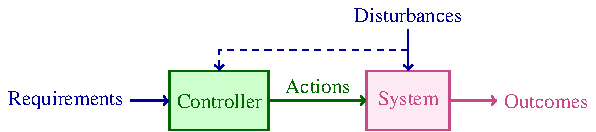
\includegraphics[width=0.60\columnwidth]{./Unit-01/img/Taxonomy-OpenLoop-scheme.pdf}
       \end{center}
 \item Requirements, \underline{system output(s)} and possibly disturbances\\
       $\Rightarrow$ \TC{closed-loop} or \TC{feedback} control, possibly with \TC{disturbance compensation}:
       \begin{center}
        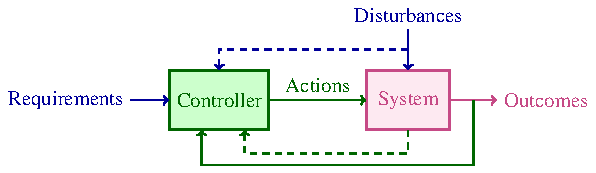
\includegraphics[width=0.60\columnwidth]{./Unit-01/img/Taxonomy-ClosedLoop-scheme.pdf}
       \end{center}
 \end{itemize}
\end{frame}

\begin{frame}\mccz
\frametitleTC{A very simple control taxonomy -- axis 2}
\framesubtitleTC{When the controller determines the control action}
\myPause
 \begin{columns}
  \column[T]{0.25\textwidth}
   \only<2 | handout:0>{\centering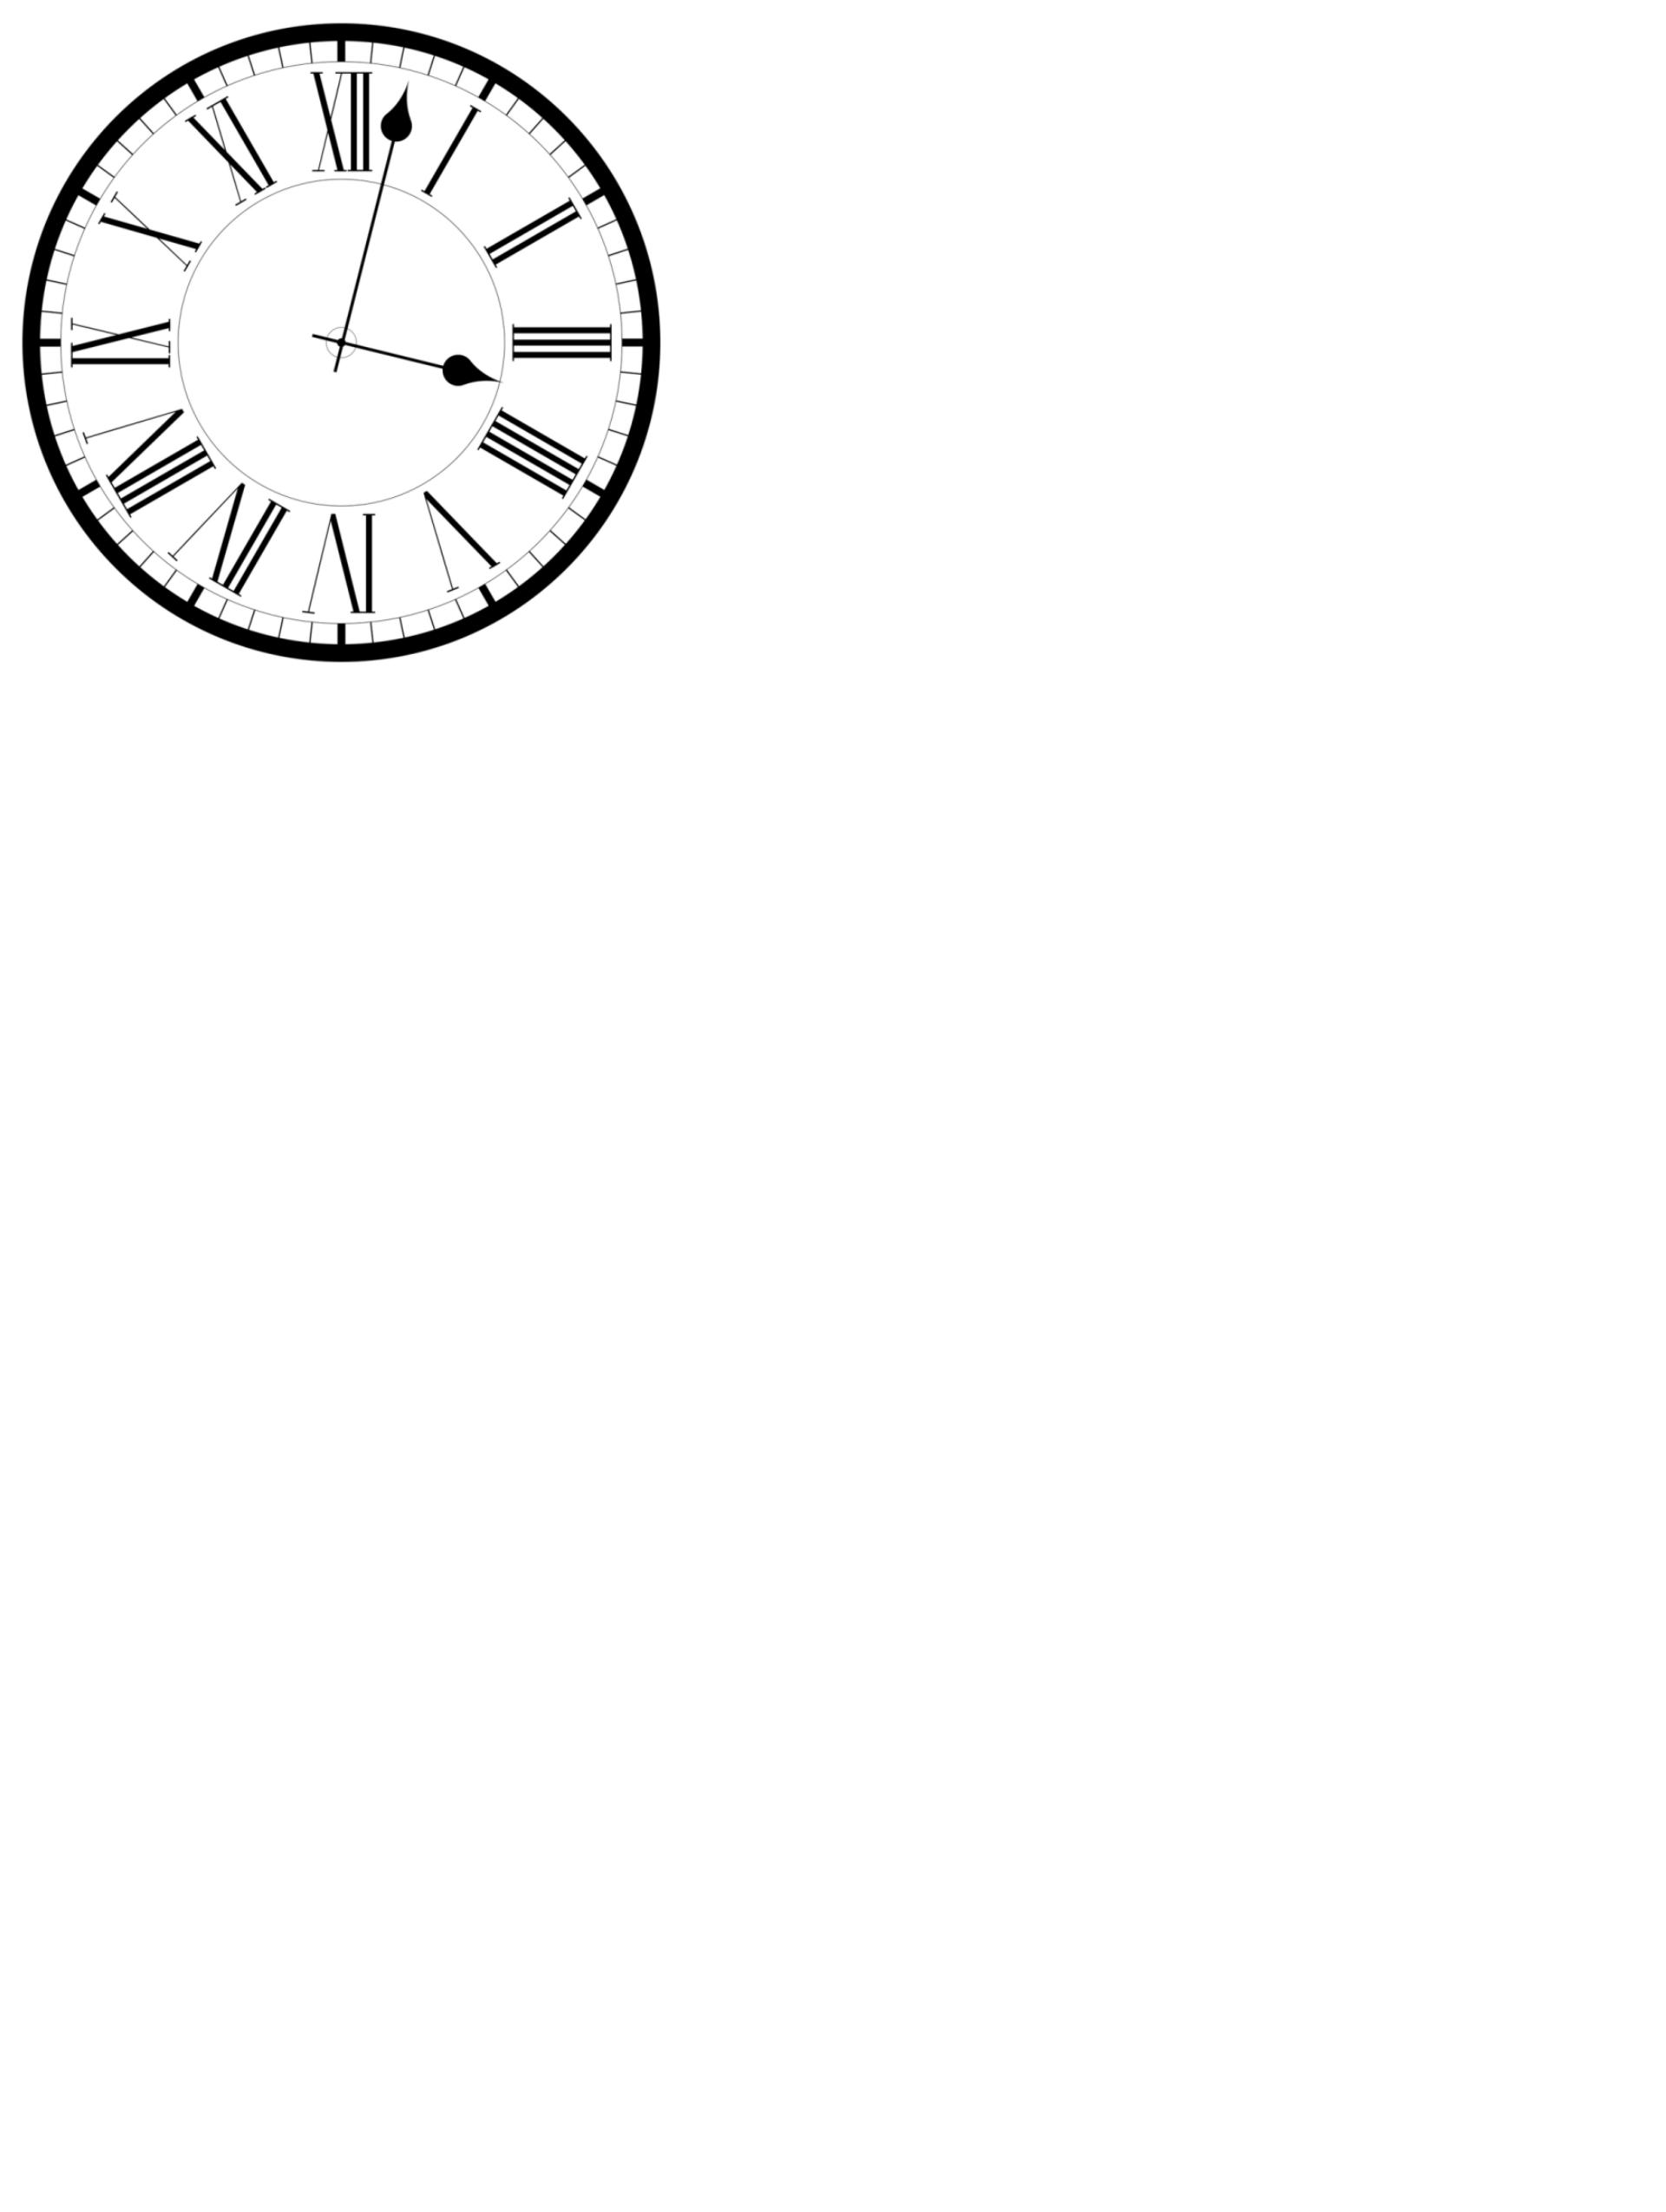
\includegraphics[height=5.5cm]{./Unit-01/img/Taxonomy-When-1_cc0.jpg}}%
   \only<3 | handout:0>{\centering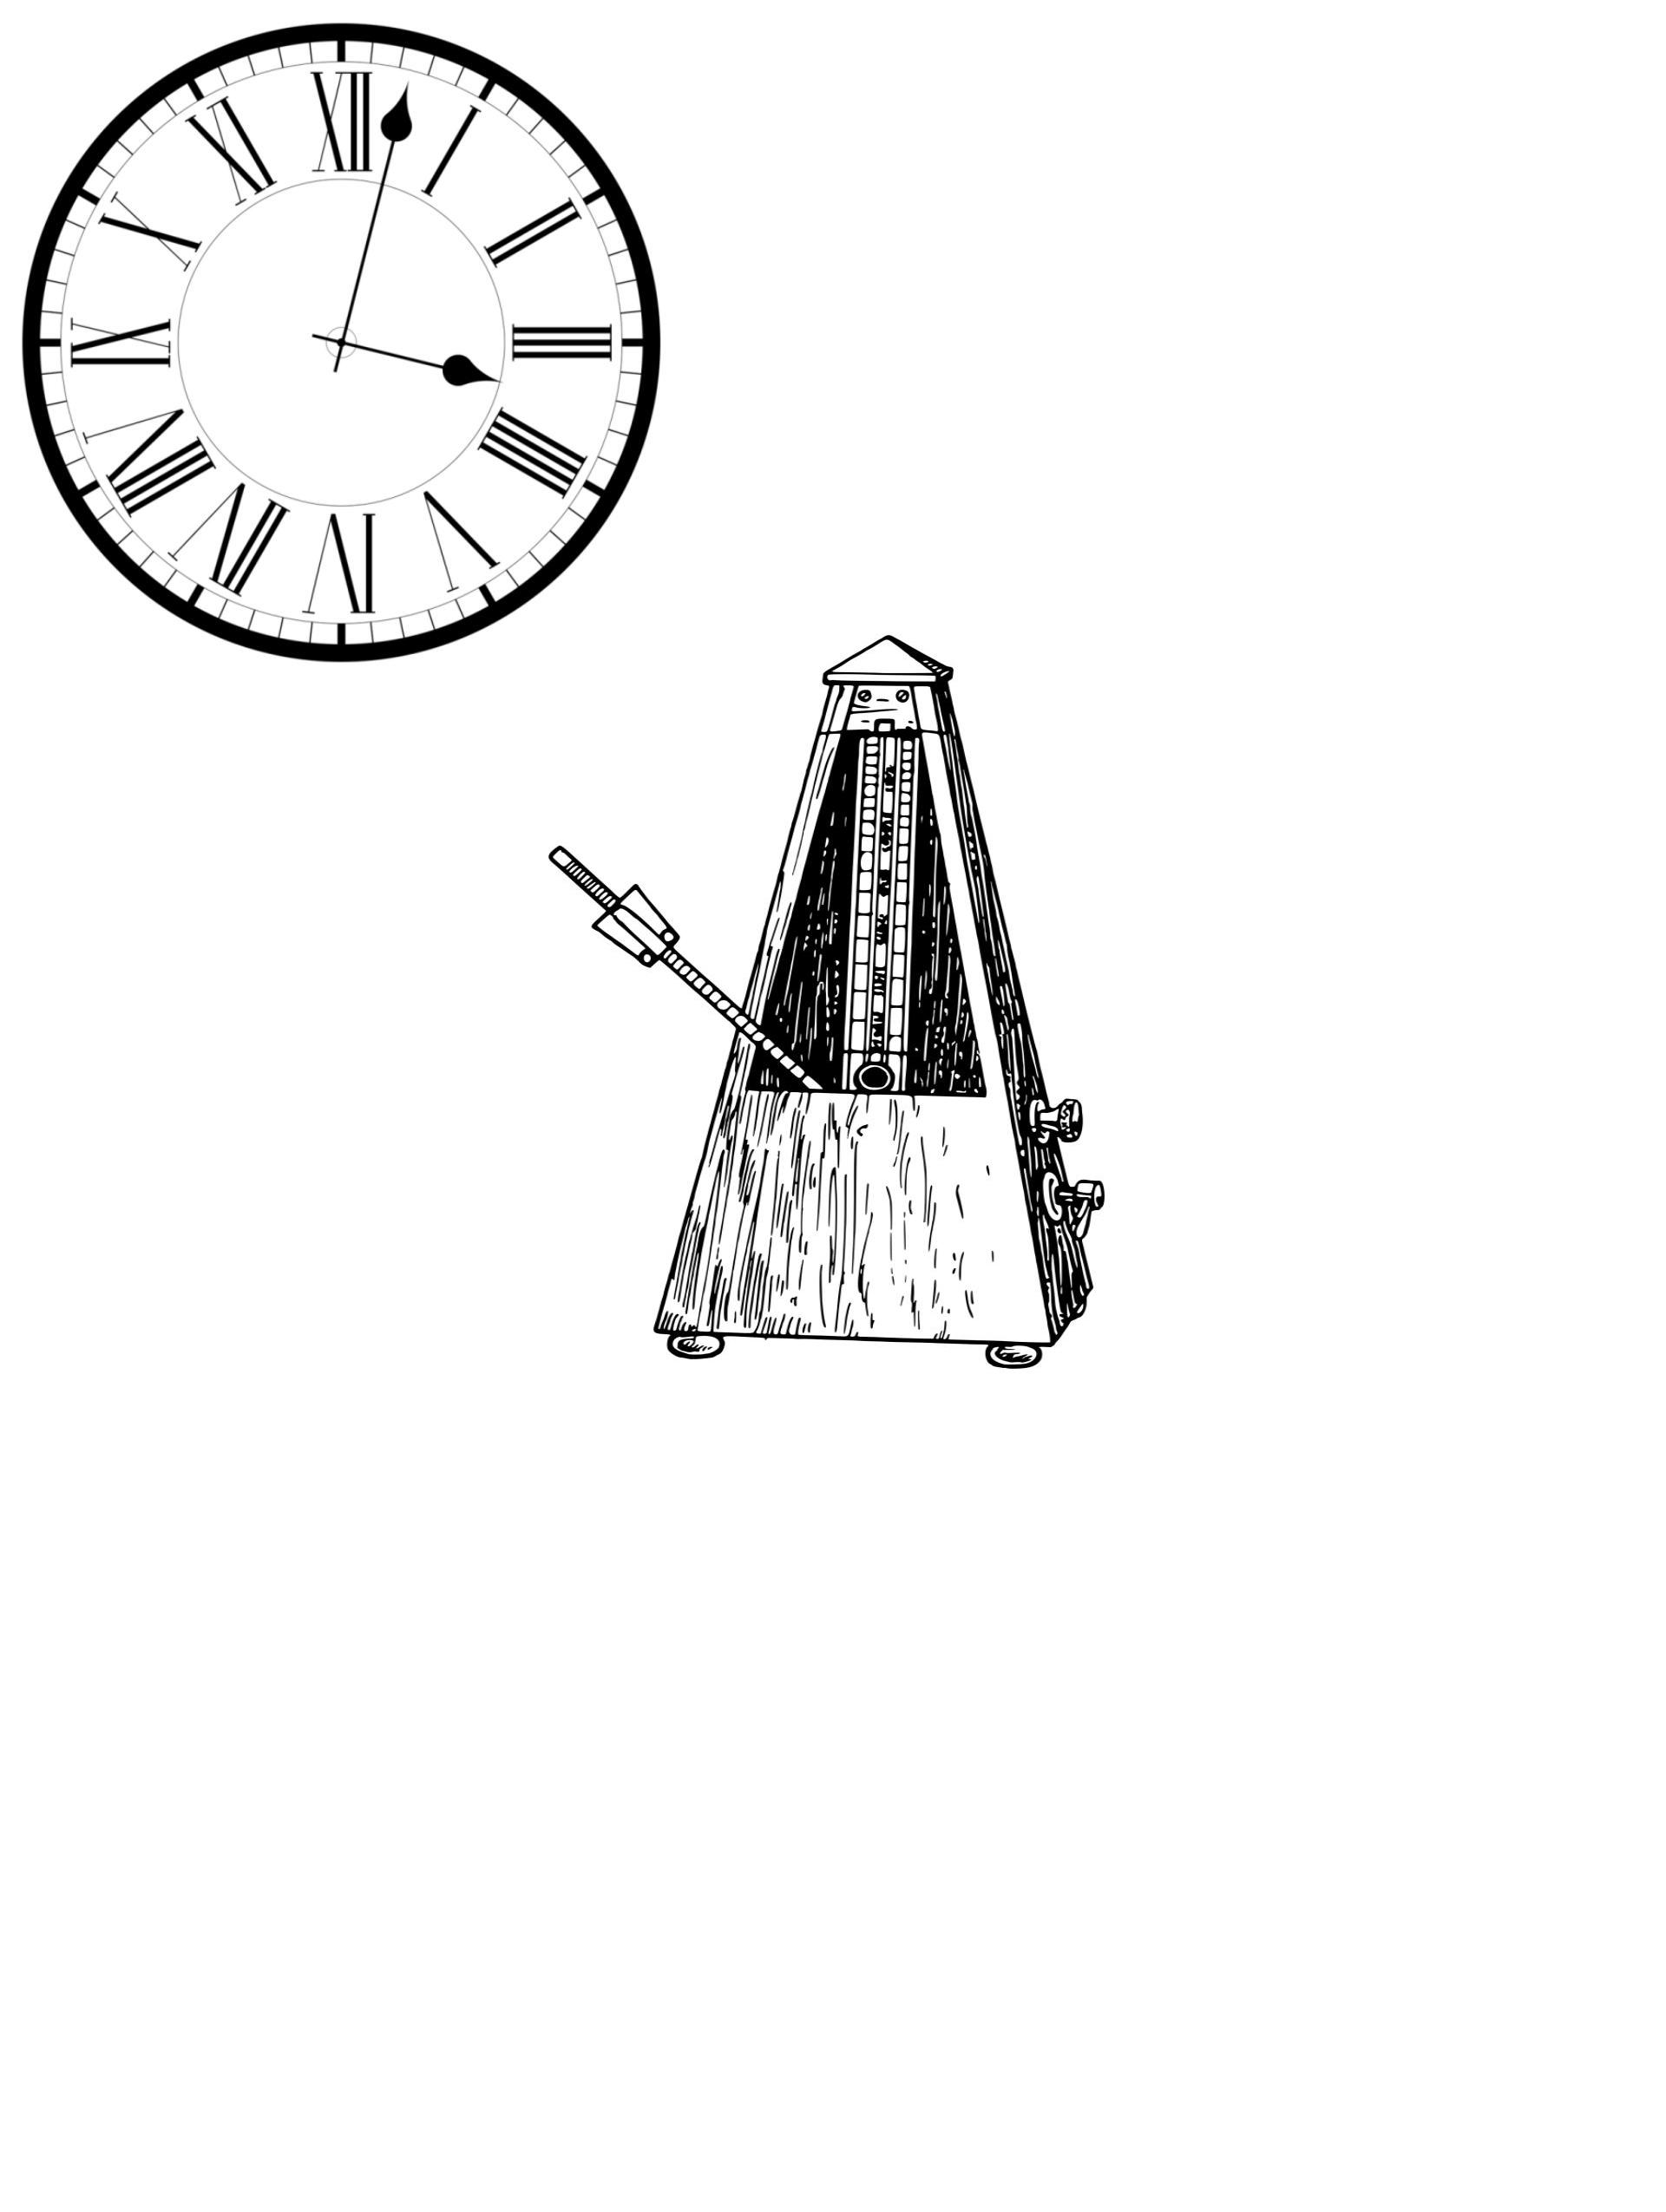
\includegraphics[height=5.5cm]{./Unit-01/img/Taxonomy-When-2_cc0.jpg}}%
   \only<4-           >{\centering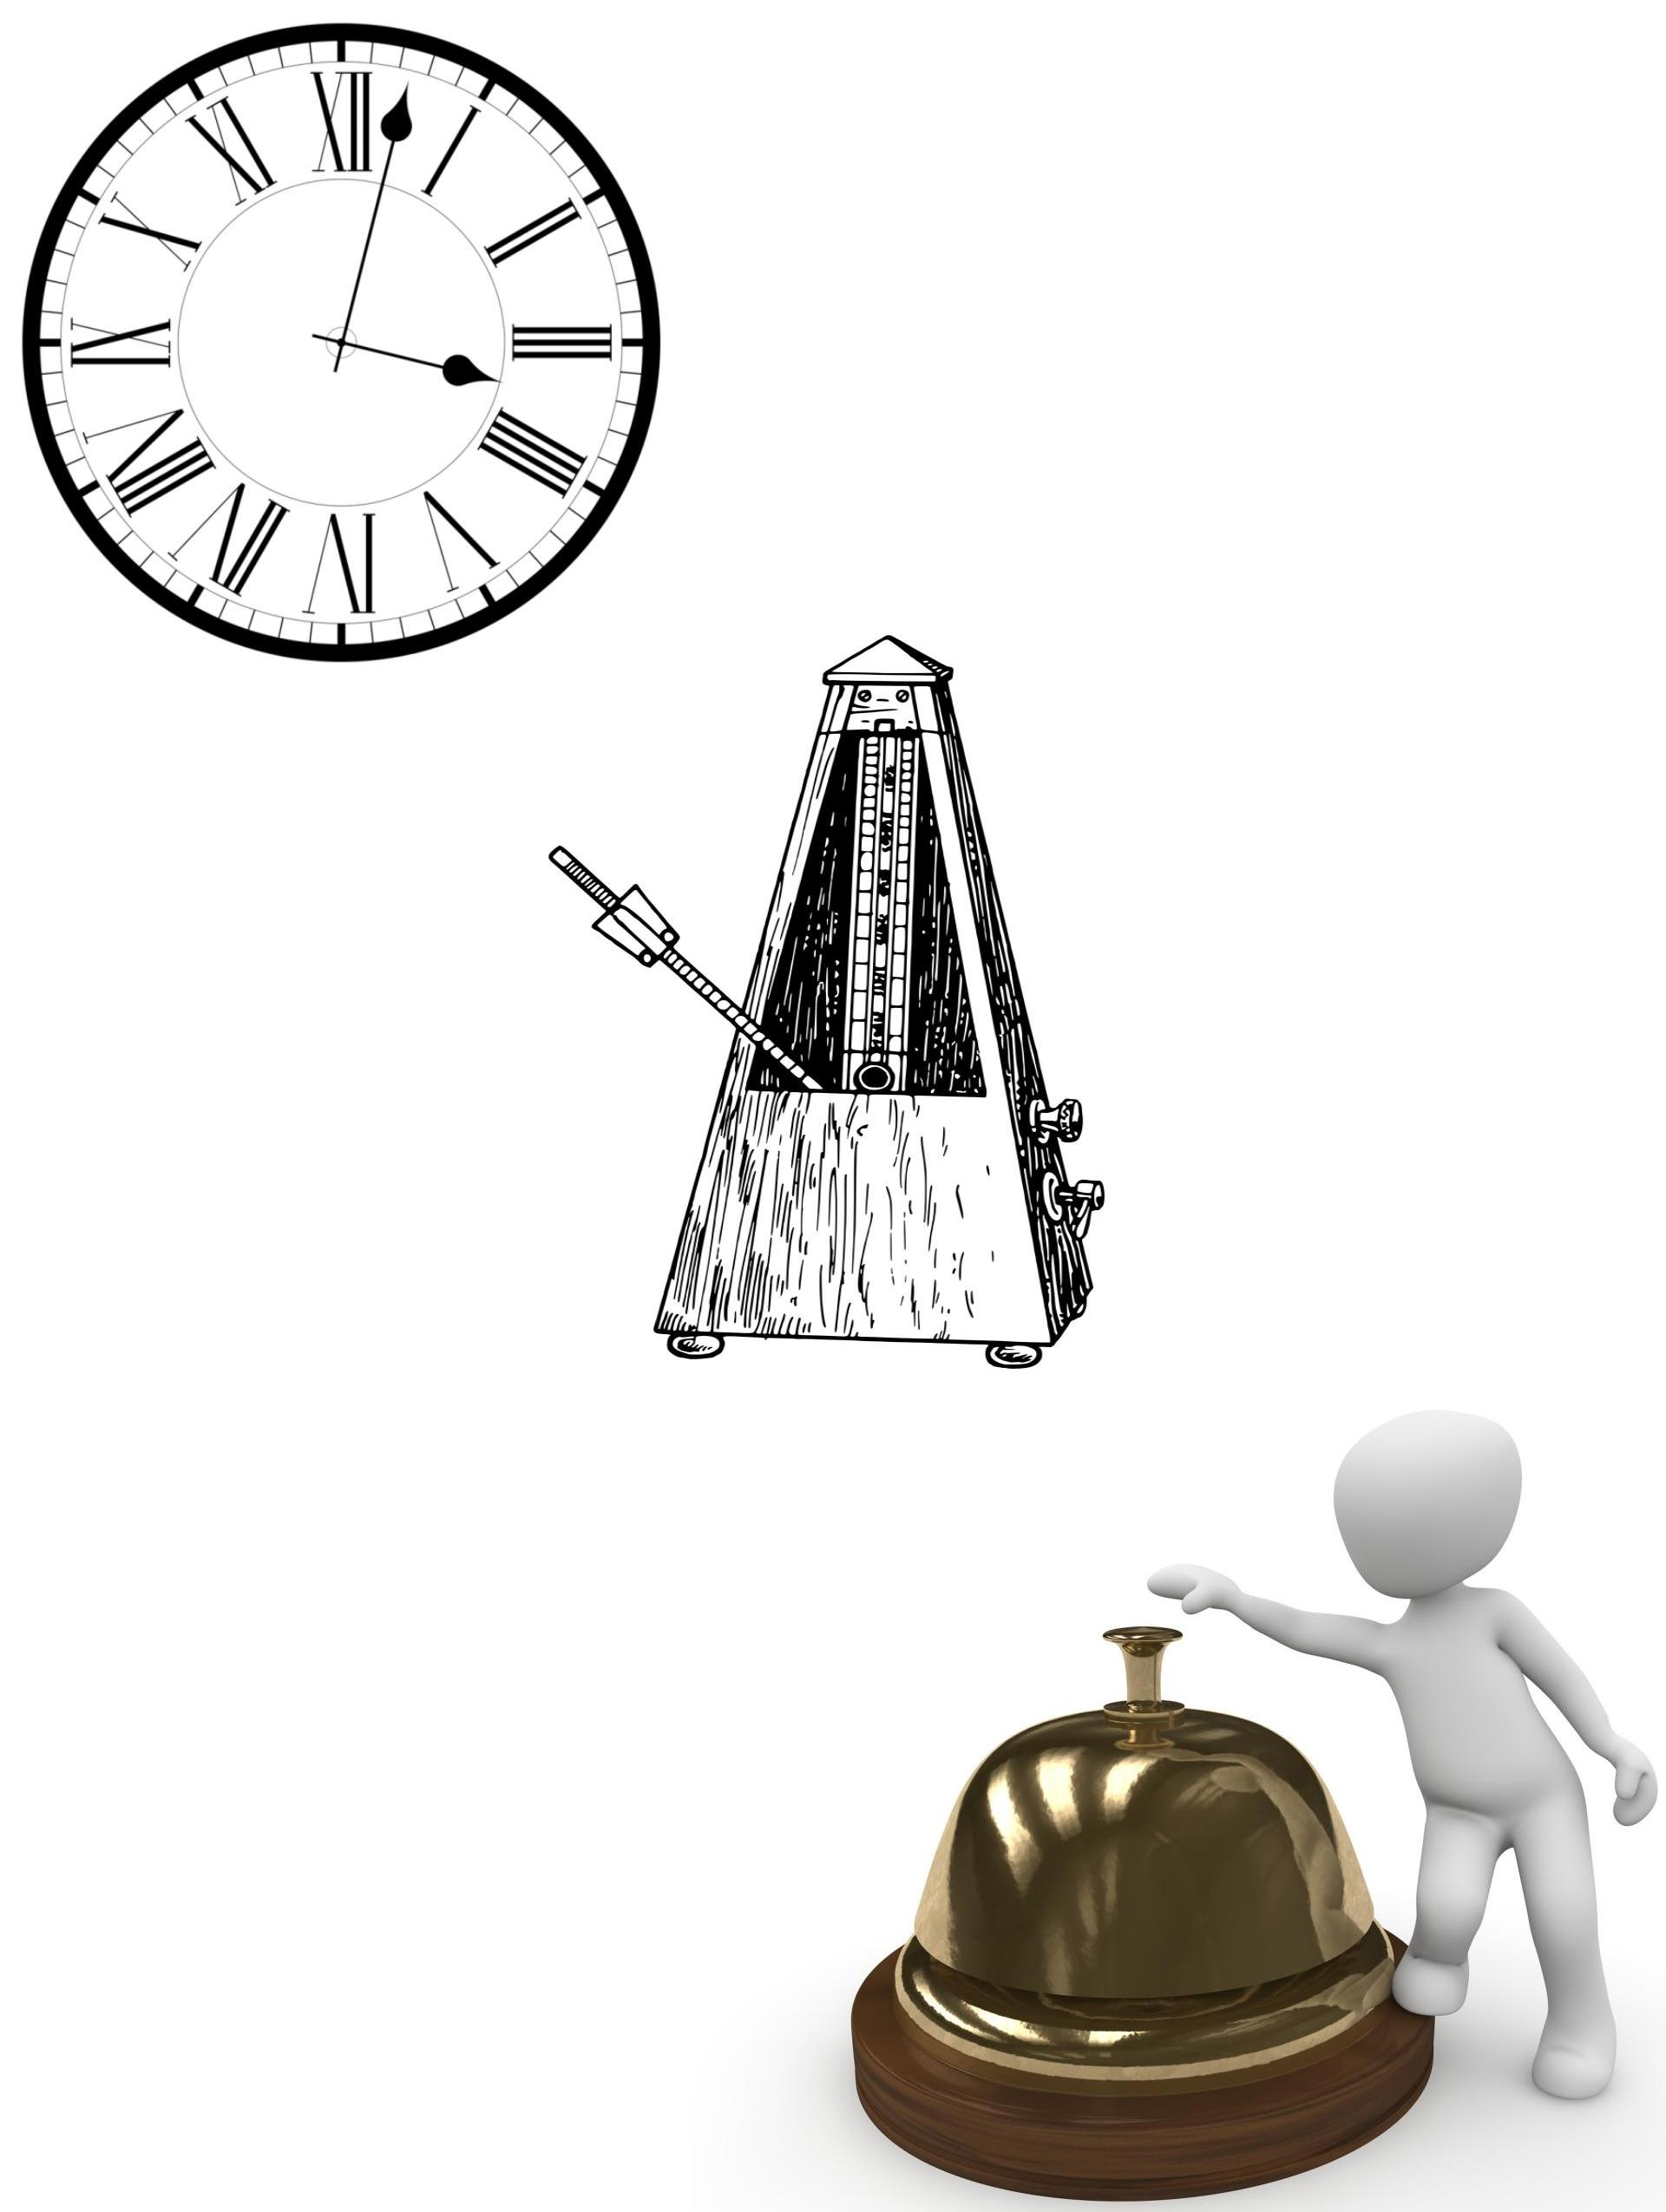
\includegraphics[height=5.5cm]{./Unit-01/img/Taxonomy-When-3_cc0.jpg}}%
  \column[T]{0.70\textwidth}
   \begin{itemize}[<+-| alert@+>]
   \item Continuously $\Rightarrow$ \TC{continuous-time} control\\
         (e.g., analogue electronics).
   \item \vspace{6mm}At points in time known \emph{a priori} $\Rightarrow$ \TC{discrete-time} control\\
         (e.g. and most typical, ISR for a \TC{periodic} interrupt).
   \item \vspace{6mm}When requested $\Rightarrow$ \TC{event-triggered} control\\
         (e.g., when a signal has changed 
          by more\\ than a given quantity wrt the last\\ control determination).
   \end{itemize}
 \end{columns}
\end{frame}

\begin{frame}\mccz
\frametitleTC{A very simple control taxonomy -- axis 3}
\framesubtitleTC{What is the nature of the control action}
\myPause
 \begin{columns}
  \column[T]{0.25\textwidth}
   \only<2 | handout:0>{\centering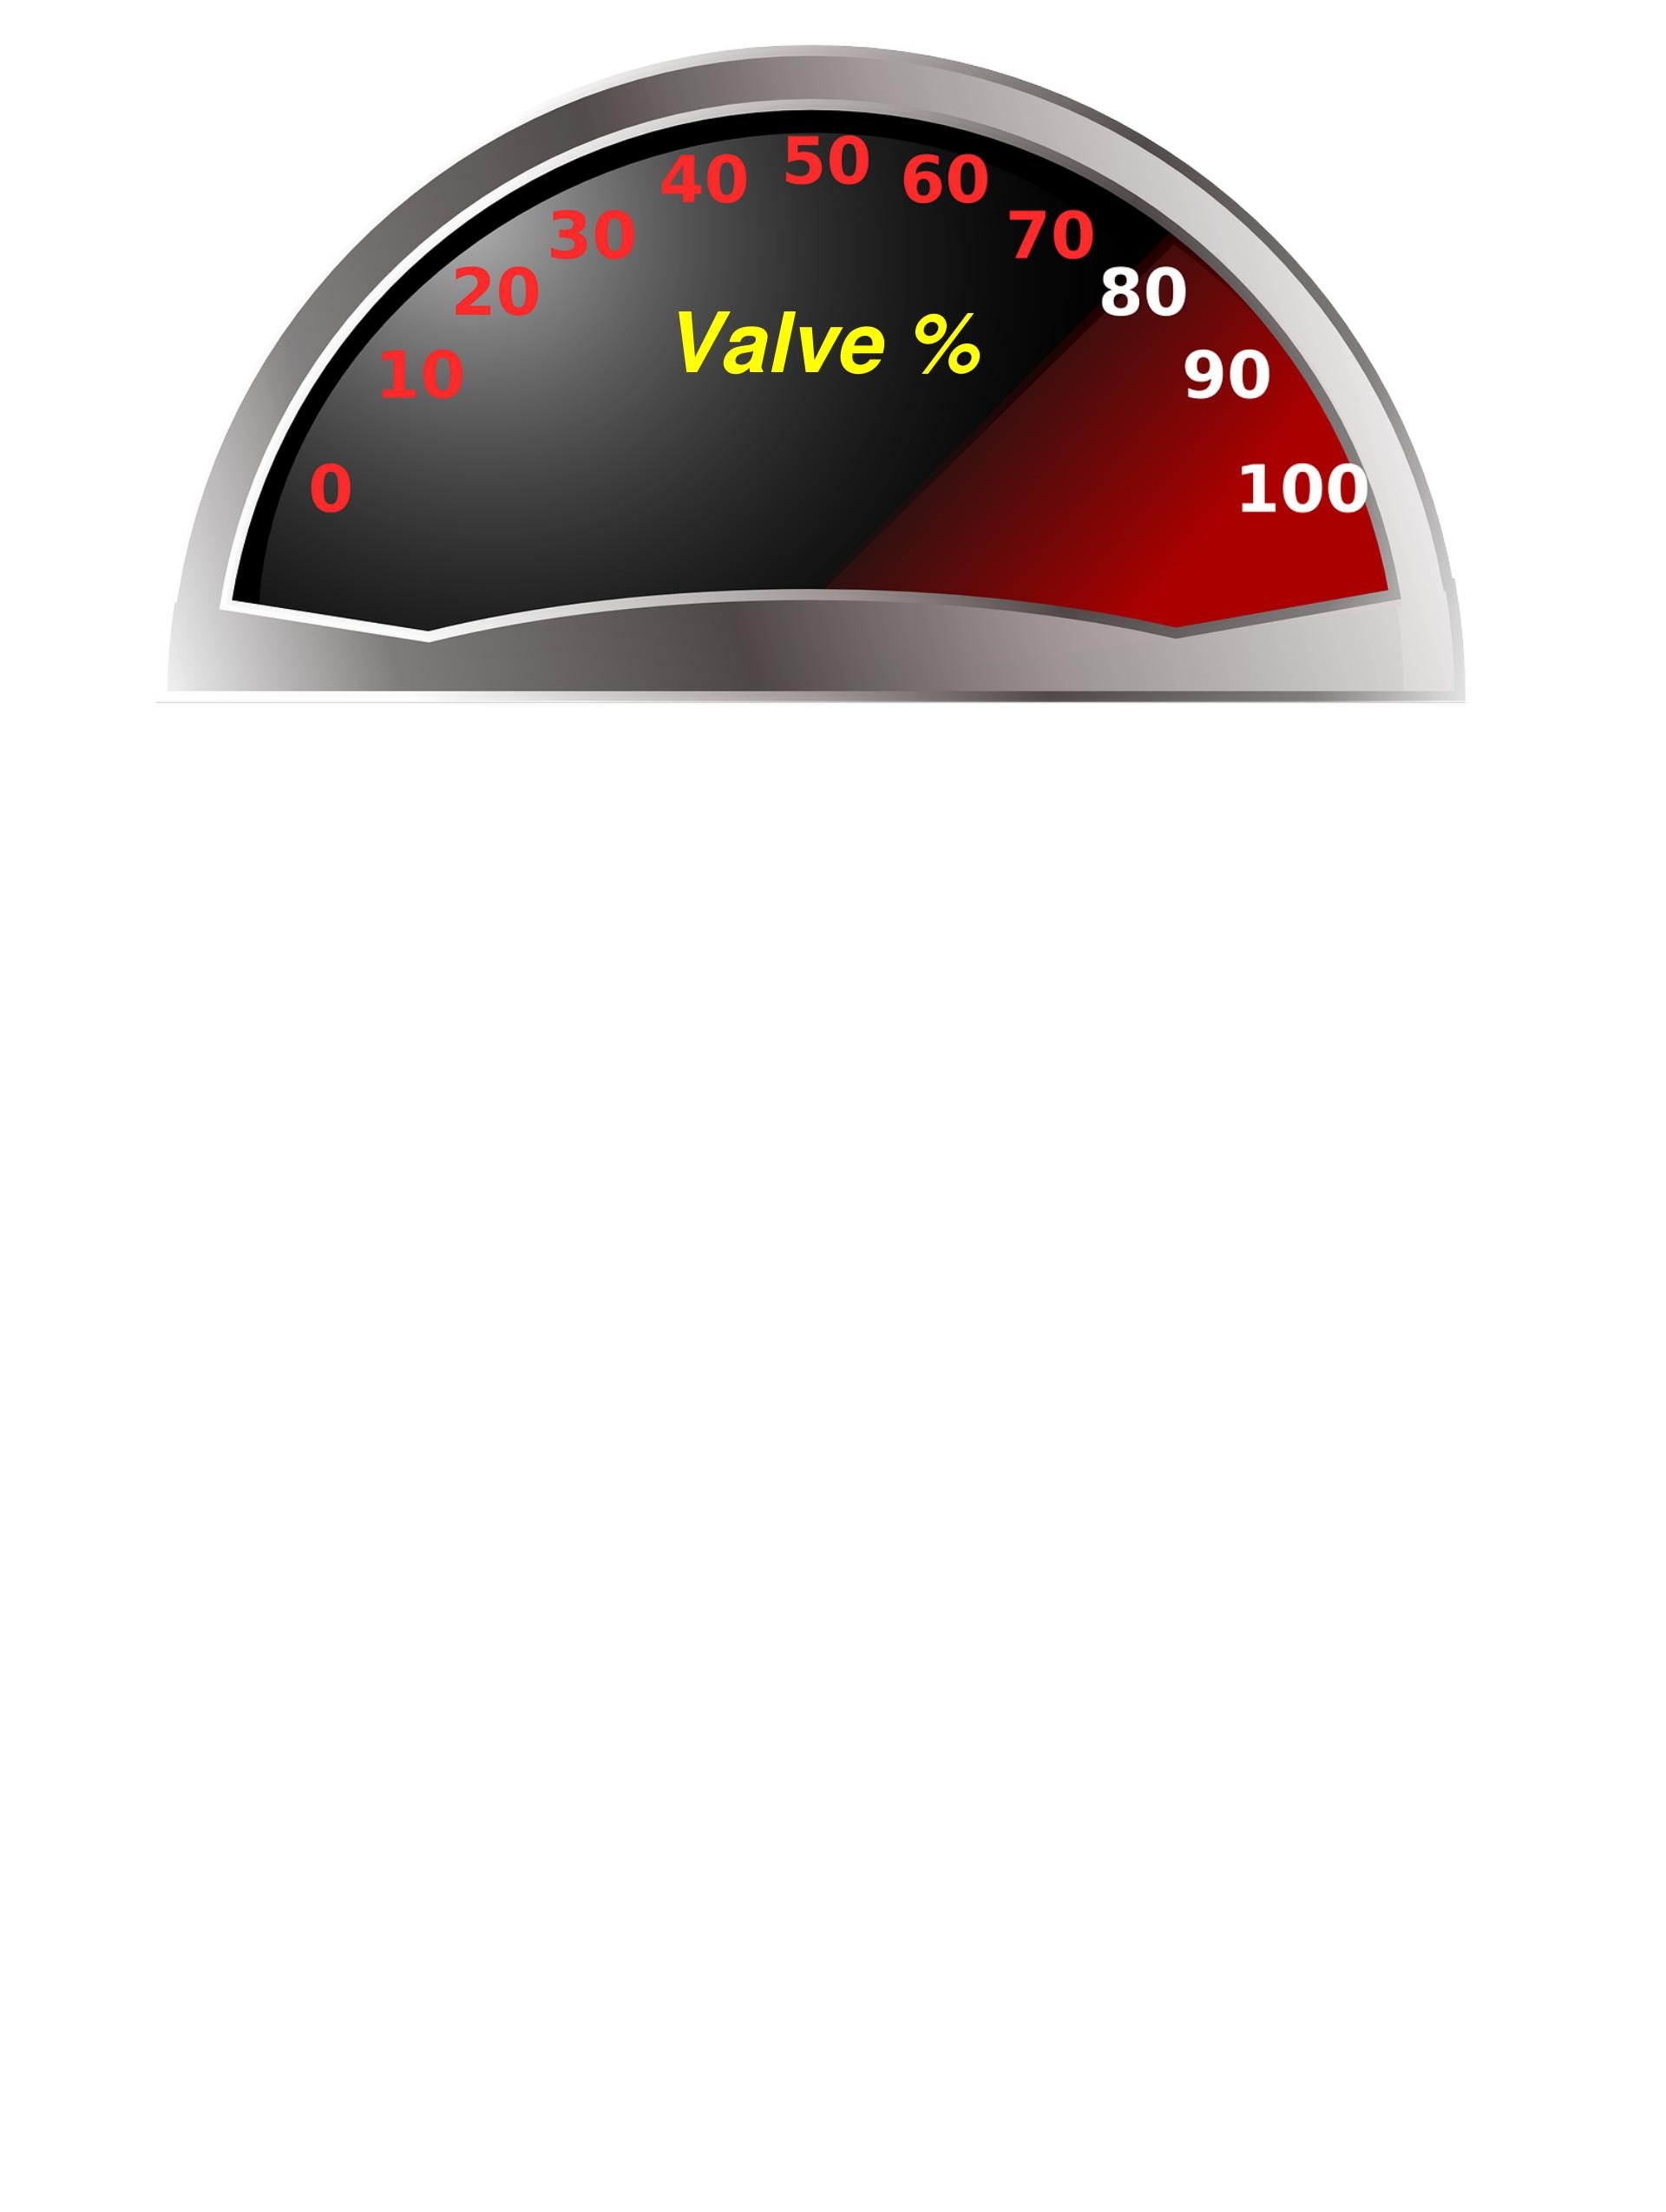
\includegraphics[height=6cm]{./Unit-01/img/Taxonomy-MvsL-1_cc0.jpg}}%
   \only<3-           >{\centering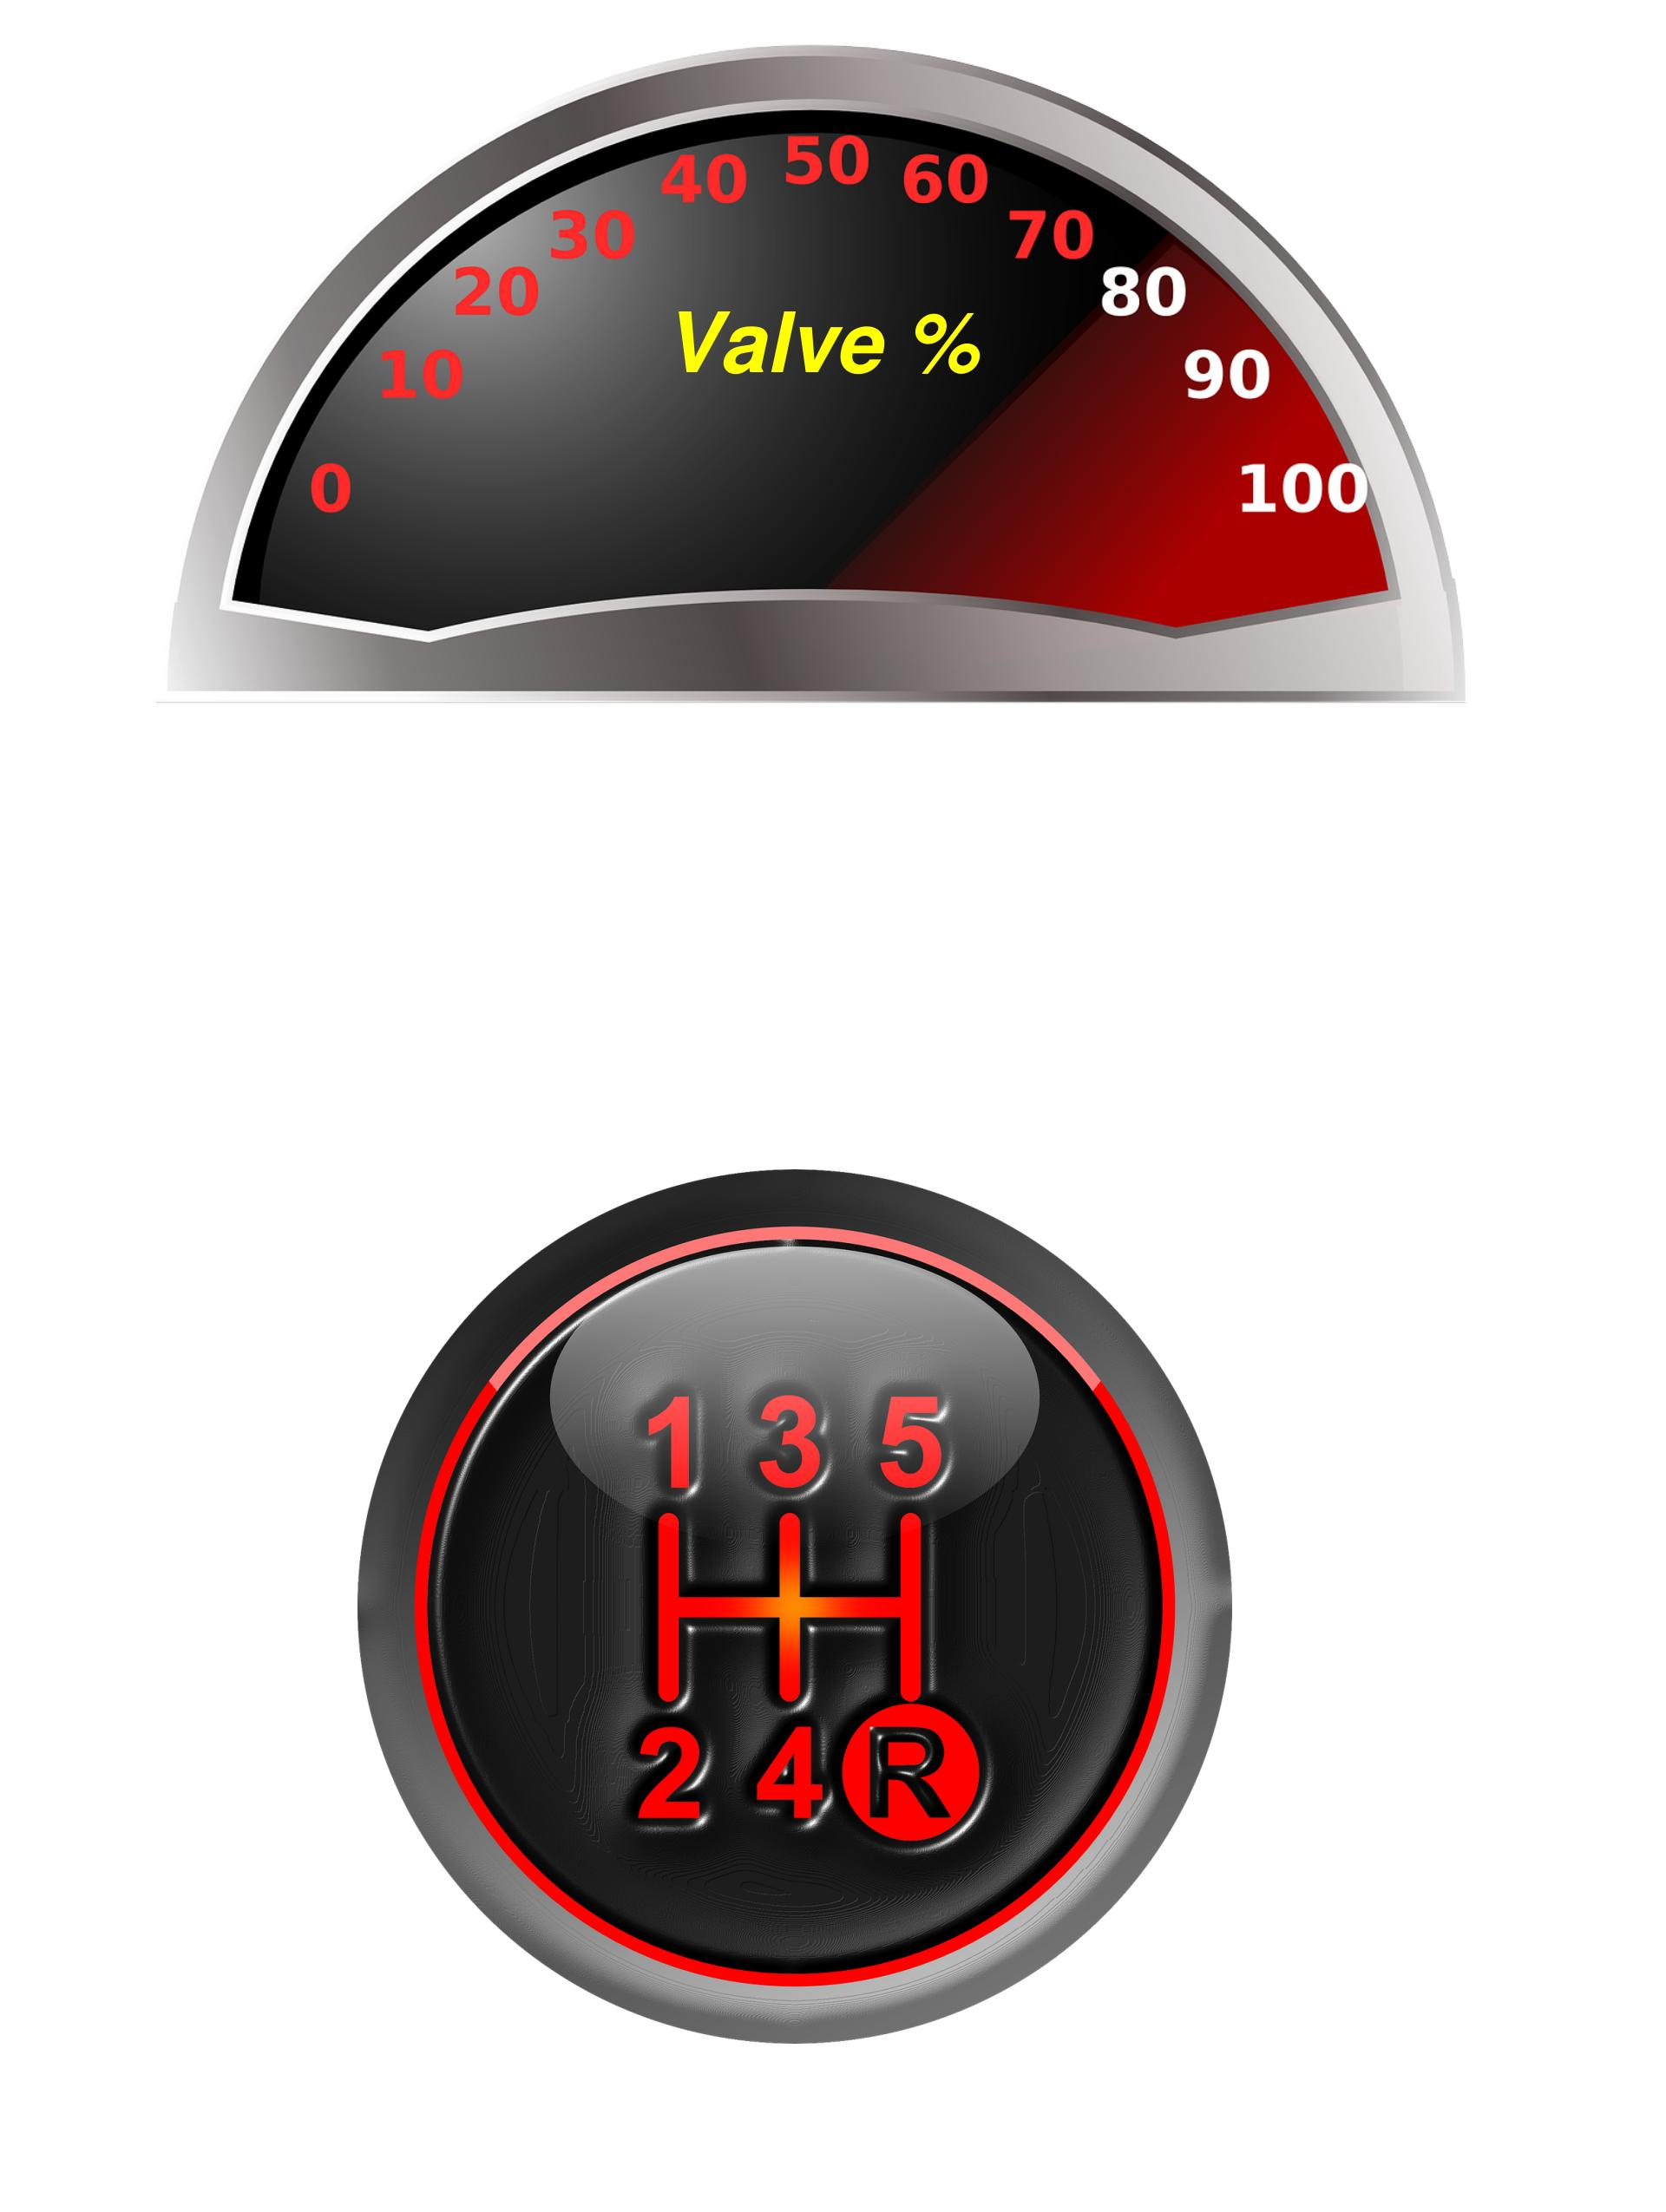
\includegraphics[height=6cm]{./Unit-01/img/Taxonomy-MvsL-2_cc0.jpg}}%
  \column[T]{0.70\textwidth}
   \begin{itemize}[<+-| alert@+>]
   \item Numeric, possibly quantised $\Rightarrow$ \TC{modulating} control\\
         (e.g., valve opening from 0 to 100\%,\\
         motor supply voltage from 0 to 24V in 0.1V steps,...);
         NOTE: \underline{any} such action has lower/upper bounds\\
         owing to physics.
   \item \vspace{10mm}Lexical ($\sim$bool/enum) $\Rightarrow$ \TC{logic} control\\
         (e.g., heater on/off,\\
          gear=\{reverse,neutral,1..5\},\\
          motor dir= \{forward,stop,backward\},...).
   \end{itemize}
 \end{columns}
\end{frame}

\begin{frame}[fragile]
\frametitleTC{Summarising}
\framesubtitleTC{brutally indeed}
\myPause
 \begin{itemize}[<+-| alert@+>]
 \item Controller:\\
         \begin{verbatim}
 type                     = {modulating,logic}
 timing                   = {continuous,discrete,event_triggered}
 connection_with_system   = {open-loop,closed_loop}
 disturbance_compensation = {present,absent}
         \end{verbatim}
 \item \vspace{-5mm}There are corner cases to this taxonomy, but for our purpose we can safely\\
       neglect them.
 \item In complex systems, controllers of different nature co-exist.
 \item \vfill To design and assess a controller, we need a modelling formalism.
 \item To make problems tractable, this formalism must also fit\\
       the controlled system.
 \item We thus move to the concept of \TC{dynamic system}.
 \end{itemize}
\end{frame}

